%************************************************
\chapter{Method}\label{ch:method}
%************************************************
\section{Data Preprocessing}

	\subsection{The TIMIT speech corpus}
		TIMIT is a speech corpus that contains phonemically transcribed speech~\citep{garofolo1993darpa}, comprising 6300 sentences, 10 spoken by each of the 630 speakers.
		To include a broad range of dialects these speakers are sampled from 8 different geographical regions in the United States (as categorized in \citet{labov2008atlas}) in which they lived during their childhood years.
		Table~\ref{tab:dialects} breaks down the precise composition of the dialect distribution.

		\begin{table}[ht]
		    \myfloatalign
		    \begin{tabularx}{\textwidth}{lrrr} \toprule
		        \tableheadline{Dialect region} & \tableheadline{\#Male}
		        & \tableheadline{\#Female} & \tableheadline{Total} \\ \midrule
		        % Phantoms take care of right-alignment (works iff monospaced digits)
		        1 (New England)   & 31 (63\%) & 18 (27\%) &  49  \phantom{0}(8\%)  \\
		        2 (Northern)      & 71 (70\%) & 31 (30\%) & 102 (16\%) \\
		        3 (North Midland) & 79 (67\%) & 23 (23\%) & 102 (16\%) \\
		        4 (South Midland) & 69 (69\%) & 31 (31\%) & 100 (16\%) \\
		        5 (Southern)      & 62 (63\%) & 36 (37\%) &  98 (16\%) \\
		        6 (New York City) & 30 (65\%) & 16 (35\%) &  46  \phantom{0}(7\%)  \\
		        7 (Western)       & 74 (74\%) & 26 (26\%) & 100 (16\%) \\
		        8                 & 22 (67\%) & 11 (33\%) &  33  \phantom{0}(5\%)  \\
		        \midrule
		        All  & 438 (70\%) & 192 (30\%) & 630 (100\%) \\
		        \bottomrule
		    \end{tabularx}
		    \caption[TIMIT Dialect Regions]{Distribution of speakers' dialect regions and sexes. Speakers of the innominate dialect region 8 relocated often during their childhood.}  \label{tab:dialects}
		\end{table}

		The sentence text can be categorized into 2 \emph{dialect} sentences, 450 \emph{phonetically compact} sentences, and 1890 \emph{phonetically diverse} sentences.

		The dialect sentences, which are spoken by all speakers, are designed to expose the dialectical variants of the speakers.
		The phonetically compact sentences are designed to include many pairs of phones.
		The phonetically diverse sentences are taken from the Brown Corpus~\citep{kucera1967computational} and the Playwrights Dialog~\citep{hultzsch1964tables} in order to maximize the number of allophones (\ie, different phones used to pronounce the same phoneme).
		Table~\ref{tab:types} lists an overview of the distribution of the number of speakers per sentence type.

		\begin{table}[ht]
		    \myfloatalign
		    \begin{tabularx}{\textwidth}{lrrrr} \toprule
		        \tableheadline{Sentence type} & \tableheadline{\#Sentences}
		        & \tableheadline{\#Speakers} & \tableheadline{Total} \\ \midrule
		        % Phantoms take care of right-alignment (works iff monospaced digits)
		        Dialect & 2    & 630 & 1260\\
		        Compact & 450  & 7   & 3150 \\
		        Diverse & 1890 & 1   & 1890 \\
		        \midrule
		        Total   & 2342 &     & 6300 \\
		        \bottomrule
		    \end{tabularx}
		    \caption[TIMIT Sentence Types]{Distribution of sentence types.}
		    \label{tab:types}
		\end{table}

		Each of the sentences is encoded in as a waveform signal in \texttt{.wav} format, and is accompanied by a corresponding text file indicating which phones are pronounced in the waveform, and between which pairs of sample points.

	\subsection{Data splitting}
		The TIMIT dataset is split into a training, validation and testing set as in \citet{graves2005framewise} and \citet{bellec2020solution}.
		The training set is used to train the network synaptic weights according to the e-prop algorithm.
		The validation set is used to obtain a well-performing set of hyperparameters.
		The testing set is used to evaluate the performance of the network after the hyperparameters are obtained.

		The TIMIT corpus documentation offers a suggested partitioning of the training and testing data, which is based on the following criteria:
		\begin{enumerate}
			\item 70\%--80\% of the data is used for training, and the remaining 20\%--30\% for testing.
			\item No speaker appears in both the training and testing portions.
			\item Both subsets include at least 1 male and 1 female speaker from every dialect region.
			\item There is a minimal overlap of text material in the two subsets.
			\item The test set should contain all phonemes in as many allophonic contexts as possible.
		\end{enumerate}
		In accordance with these criteria, the TIMIT corpus includes a ``core'' test set that contains 2 male speakers and 1 female speaker from each dialect, summing up to 24 speakers.
		Each of these speakers read a different set of 5 phonetically compact sentences, and 3 phonetically diverse sentences that were unique for each speaker.
		Consequently, the test set comprises 192 sentences ($24\times(5+3)$) and was selected such that it contains at least one occurrence of each phoneme.
		In this report, the TIMIT core test set is used, thereby meeting the criteria listed above.

		The remaining 4096 sentences are randomly partitioned into 3696 training sentences and 400 validation sentences in this research (the TIMIT corpus contains no fixed training/validation set partition).

	\subsection{Engineering features}

		The data preprocessing pipeline is similar to that used in \citet{fayek2016}, which can be summarized by applying a pre-emphasis filter on the waveforms, then slicing the waveform in short frames, taking their short-term power spectra, computing 26 filterbanks, and finally obtain 12 Mel-Frequency Cepstrum Coefficients (MFCCs).
		Then, these MFCCs are aligned with the phones found in the TIMIT dataset.
		An example of a waveform signal is given in Figure \ref{fig:signal}.
			\begin{figure}[ht]
				\centering
			    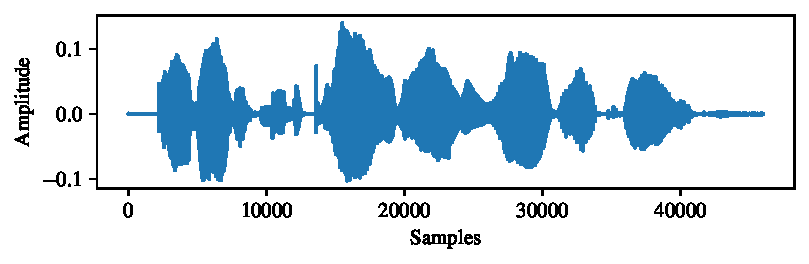
\includegraphics[width=\linewidth]{gfx/signal}
			    \caption{A raw waveform signal from the TIMIT dataset.}
			    \label{fig:signal}
			\end{figure}

		\paragraph{Pre-emphasis}

			In speech signals, high frequencies generally have smaller magnitudes than lower frequencies.
			To balance the magnitudes over the range of frequencies in the signal, a pre-emphasis filter $y(t)$ is applied on the waveform signal $x(t)$ defined in Equation \ref{eq:pre_emphasis}.
			\begin{equation}\label{eq:pre_emphasis}
				y(t) = x(t) - 0.97x(t-1)
			\end{equation}
			This procedure yields the additional benefit of improving the signal-to-noise ratio.
			An example of a pre-emphasized signal is given in Figure \ref{fig:signalemph}.
			\begin{figure}[ht]
				\centering
			    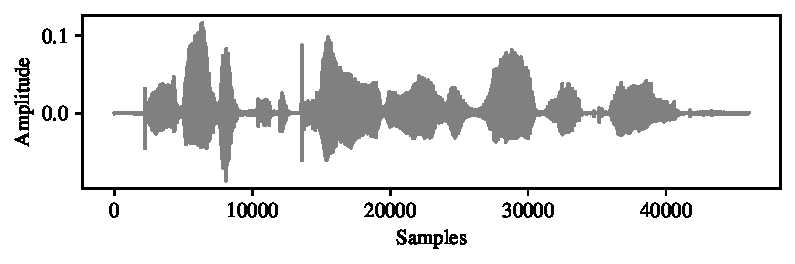
\includegraphics[width=\linewidth]{gfx/signalemph}
			    \caption[Pre-emphasis]{A signal after the pre-emphasis filter of Equation \ref{eq:pre_emphasis} was applied to it.}
			    \label{fig:signalemph}
			\end{figure}

		\paragraph{Framing}
			The waveforms, which are sampled at a rate $f_s$ of \SI{16}{\kHz}, cannot be directly used as input to the model, because they are too long---a typical sentence waveform contains in the order of tens of thousands of data points.
			Furthermore, the individual data points are not very informative, because they reflect the sound wave of the uttered sound, not the characteristics of the source of this sound.
			These sounds are filtered by the shape of the vocal tract, which manifests itself in the envelope of the short time power spectrum of the sound.
			This power spectrum representation describes the power of the frequency components of the signal over a brief interval.
			The frequency components are assumed to be stationary over short intervals, in contrast to the full sentence, which carries its meaning because it is non-stationary.
			Therefore, the waveform signals are transformed into series of frequency coefficients of short-term power spectra.
			To obtain these multiple short-term power spectra over the duration of the waveform, it is sliced into brief overlapping frames.

			Every 160 samples (equivalent to \SI{10}{ms}) of a pre-emphasized signal, an interval frame of 400 samples (equivalent to \SI{25}{ms}) is extracted.
			This means that the frames overlap by \SI{25}{ms}.
			The waveform is zero-padded such that the last frame also has 400 samples.
			By this process, signal frames $x_i(n)$ are obtained, where $n$ ranges over 1--400, and $i$ ranges over the number of frames in the waveform.

			Then, a Hamming window with the form
			\begin{equation}\label{eq:hamming}
				w\left[n\right] = a_0 - a_1\cos\left(\frac{2\pi n}{N-1}\right),
			\end{equation}
			is applied where $N$ is the window length of 400 samples, $0 \leq n < N$, $a_0 = 0.53836$, and $a_1 = 0.46164$.
			A plot of this window is given in Figure \ref{fig:hamming}.
			\begin{figure}[ht]
				\centering
			    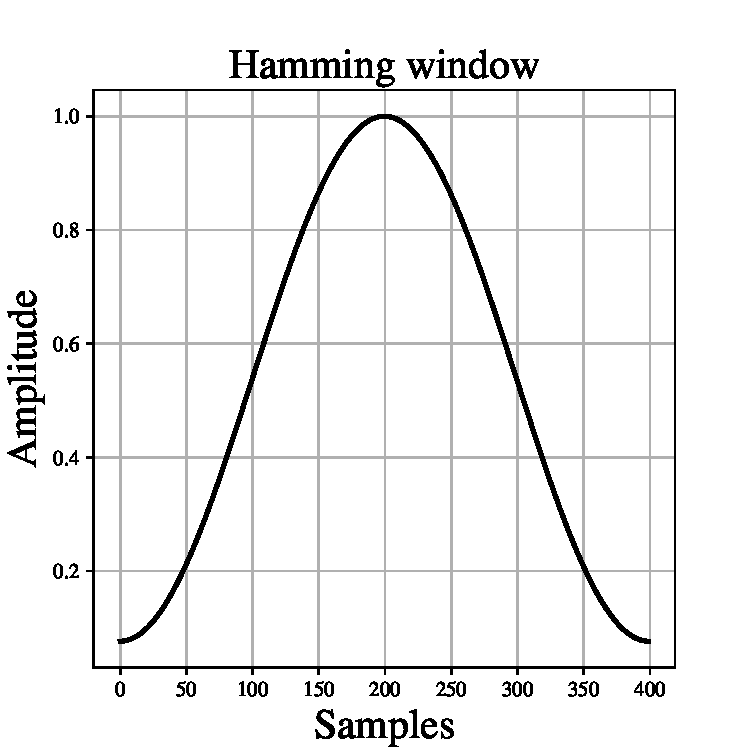
\includegraphics[width=0.45\linewidth]{gfx/hamming}
			    \caption{The form of the Hamming window applied on signal frames to reduce spectral leakage.}
			    \label{fig:hamming}
			\end{figure}
			This window is applied to reduce the spectral leakage, which manifests itself though sidelobes in the power spectra.
			Applying the Hamming window reduces the sidelobes to near-equiripple conditions, minimizing the leakage \citep{SASPWEB2011}.

		\paragraph{Short-term power spectra}

			The power spectra $P_i$ are obtained for each frame by first taking the absolute $K$-point discrete Fourier transform (DFT) of the frame samples $x_i(n)$:
			% \todo{don't bother with eqn, just call mathbb(F)}
			\begin{equation}
				X_k = \left|\sum_{n=0}^{N-1}x_i(n)\cdot e^{-\frac{i2\pi}{N}kn}\right|,
			\end{equation}
			where $K=512$.
			This yields the magnitudes of the discrete cosine transform (DCT) of the frames.

			The power spectra are obtained using the equation
			\begin{equation}\label{eq:powframes}
				P = \frac{{X_k}^2}{K},
			\end{equation}
			an example of which is shown in Figure \ref{fig:powframes}.

			\begin{figure}[ht]
				\centering
			    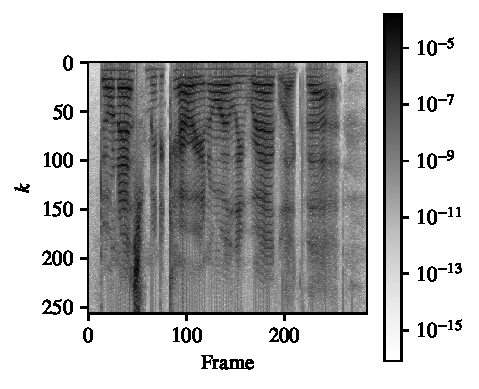
\includegraphics[width=0.45\linewidth]{gfx/powframes}
			    \caption{The power spectra of a sentence.}
			    \label{fig:powframes}
			\end{figure}

		\paragraph{Mel filterbank}

			The short-term power spectra are then transformed to Mel-spaced filterbanks.
			The Mel scale is a scale of pitches that are perceptually equal in distance \citep{stevens1937scale}.
			This is in contrast to the frequency measurement, in which the human cochlea can distinguish lower frequencies more accurately than higher ones.
			The aim of converting to the Mel scale is to make every filterbank coefficient feature equally informative, thereby improving the learning performance of the model.

			The Mel-spaced filterbank is a set of 40 triangular filters that we apply to each frame in $P$.

			To compute the Mel-spaced filterbank, lower and upper band edges of respectively \SI{0}{\Hz} and $f_s/2 = \SI{8}{\kHz}$ are selected, and convert these to Mels using
			\begin{equation}
				m(f) = 2595\log_{10}\left(1 + \frac{f}{700}\right),
			\end{equation}
			where $f$ is the frequency in $\SI{}{\Hz}$.
			This yields a lower band edge of 0 Mels and an upper band edge of approximately 2835 Mels.

			The 40 filterbanks are obtained by first spacing 42 points $\mathbf{m}$ linearly between these bounds (inclusive), thereby obtaining 40 points spaced exclusively between the bounds.

			Then, each point $m$ is converted back to \SI{}{\Hz} using
			\begin{equation}
				f = 700\left(10^{m/2595}-1\right).
			\end{equation}
			Resulting Mel-spaced frequencies $f$ are rounded to their nearest Fourier transform bin $b$ using
			\begin{equation}
				b = \lfloor(K+1)\mathbf{f}/fs\rfloor.
			\end{equation}

			The resulting 40 filterbanks with their corresponding Mels and frequencies are listed in Table \ref{tab:mels}.

			The $i\textsuperscript{th}$ filter in filterbank $H_i$ is a triangular filter that has its lower boundary at $b_{i}$ \SI{}{\Hz}, its peak at $b_{i+1}$ \SI{}{\Hz}, and its upper boundary at $b_{i+2}$ \SI{}{\Hz}.
			For other frequencies, they are 0.
			Therefore, the filterbank can be described by
			\begin{equation}
				H_i(k) = \begin{cases}
					0 & k<b_i\\
					\frac{k-b_i}{b_{i+1}-b_i} & b_i\leq k < b_{i+1} \\
					1 & k = b_{i+1} \\
					\frac{b_{i+2} - k}{b_{i+2}-b_{i+1}} & b_{i+1} < k \leq b_{i+2}\\
					0 & b_{i+2} < k
				\end{cases},
			\end{equation}
			where $0 \leq k \leq \frac{K}{2}$.
			These Mel-spaced filters are shown in Figure \ref{fig:filterbank}.
			\begin{figure}[ht]
				\centering
			    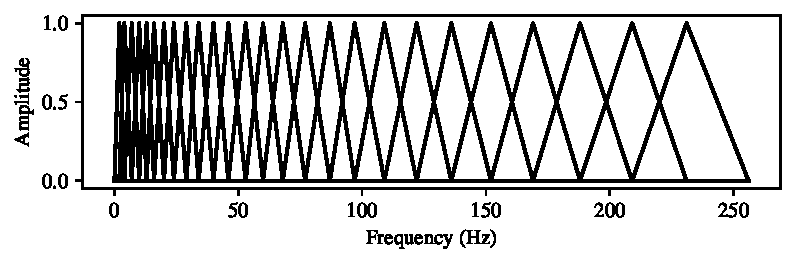
\includegraphics[width=\linewidth]{gfx/fbanks}
			    \caption{The Mel-spaced filterbanks.}
			    \label{fig:filterbank}
			\end{figure}

			After applying the filterbank to the short-term power spectrum, a spectrogram $S$ of the frame sequence (see \eg~Figure \ref{fig:spectrogram}) is obtained.

			\begin{figure}[ht]
				\centering
			    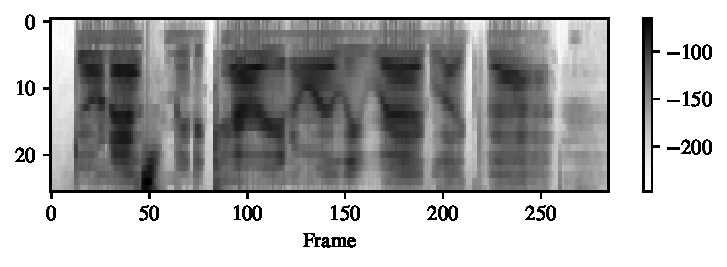
\includegraphics[width=\linewidth]{gfx/spectrogram}
			    \caption{An example of the spectrogram of a sentence.}
			    \label{fig:spectrogram}
			\end{figure}

		\paragraph{Mel-frequency cepstral coefficients}

			Coefficients in the spectrograms are strongly correlated, which would negatively impact the learning performance of the model.
			Therefore, the DCT is applied again to decorrelate the coefficients and obtain the power cepstrum $C$ of the speech frame:

			% \begin{equation}
			% 	C(n) = \left|\sum_{n=0}^{N-1}S(n)\cdot e^{-\frac{i2\pi}{N}kn}\right|.
			% \end{equation}

			\begin{equation}
				C_k = 2c\sum^{N-1}_{n=0}S\left(n\right)\cos\left(\frac{\pi k\left(2n+1\right)}{2N}\right),
			\end{equation}
			where $c$ is a scaling factor that makes the matrix of coefficients orthonormal:
			\begin{equation}
			c = \begin{cases}
				\sqrt{\frac{1}{4N}} & \mbox{if } k = 0,\\
				\sqrt{\frac{1}{2N}} & \mbox{otherwise.}
			\end{cases}
			\end{equation}

			The first coefficient in $C$ is discarded, because it indicates the average power of the input signal and therefore carries little meaning.
			Coefficients higher than 13 are also discarded, because they represent only fast changes in the spectrogram and increase the complexity of the input signal while adding increasingly less meaning to it.

			Then, the final MFCCs are balanced by centering each frame around the value 0.
			An example of the final MFCCs is given in Figure \ref{fig:source_mfcc_target}.

			\begin{figure}[ht]
			    \myfloatalign
			    \subfloat[The raw speech input signal.]
			    {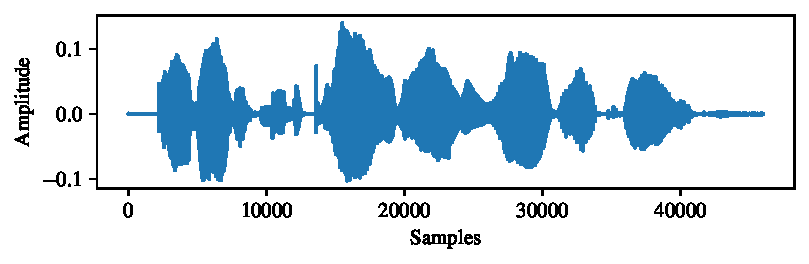
\includegraphics[width=\linewidth]{gfx/signal}} \\
			    \subfloat[MFCCs centered around 0 per channel. Note that these MFCCs are standardized channel-wise over the full training dataset.]
			    {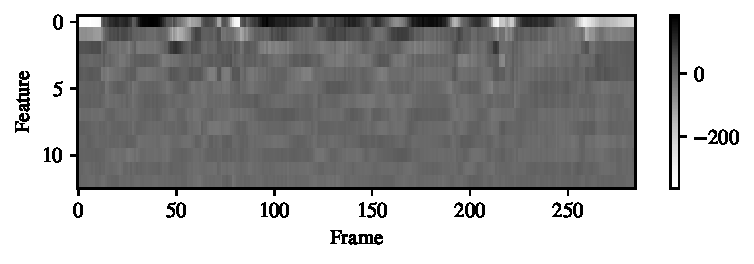
\includegraphics[width=\linewidth]{gfx/norm_mfcc}} \\
			    \subfloat[Target signal encoded as a one-hot vector changing over time. The order of phones along the one-hot vector corresponds to the order in which they are encountered in processing the dataset. This particular example shows a pattern because it is the first processed sentence in the training set.]
			    {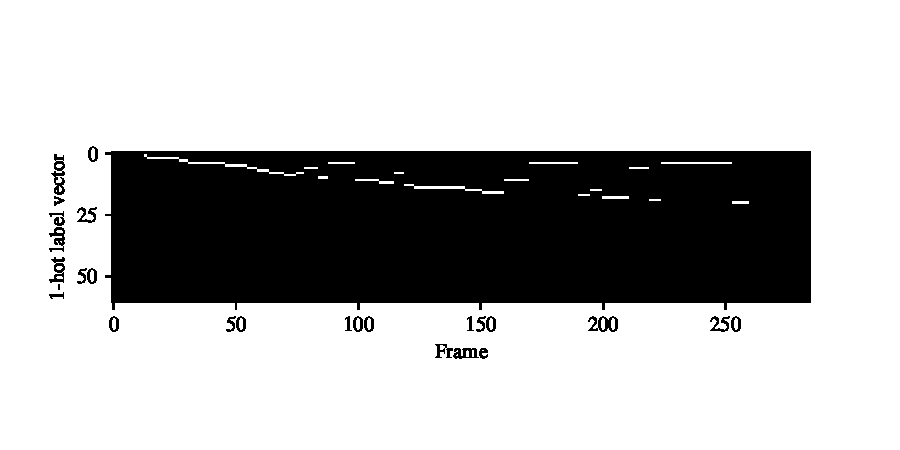
\includegraphics[width=\linewidth]{gfx/target}}
			    \caption[Input/features/targets]{An alignment of a sample signal with its MFCCs features and target phones.}\label{fig:source_mfcc_target}
			\end{figure}

		\paragraph{Target output}

			The target output of the model is a frame-wise representation of the phones that are uttered in a sentence.
			The TIMIT corpus contains text files indicating in what order phones occur in a sentence, and their starting and ending sample points.

			These phones are discretized into frames such that they align correctly with the MFCCs.
			They are represented in one-hot vector encoding.
			Since the dataset contains 61 different phones, this is also the length of these vectors.

			Figure \ref{fig:source_mfcc_target} illustrates the waveform data and its frame-wise aligned MFCCs and target output.
			Note that the full dataset of features is standardized per training data channel; feature channels are first centered around 0, and then divided by their standard deviations.
			To prevent data leakage, validation and testing data are standardized according to the means and standard deviations in the training data.
			An example of a standardized input is shown in Figure \ref{fig:inoutpair}.

\section{Enhancing e-prop}

	In this report, two types of enhancements to apply the e-prop learning algorithm on the TIMIT dataset are examined.

	The first type is the effect of the neuron model; particularly, the effect of including STDP behavior is analyzed.
	The second type is the effect of a multi-layered architecture.

	\subsection{Multi-layer architecture}\label{sec:ml_arch}

		\begin{figure}[!ht]
		    \myfloatalign
		    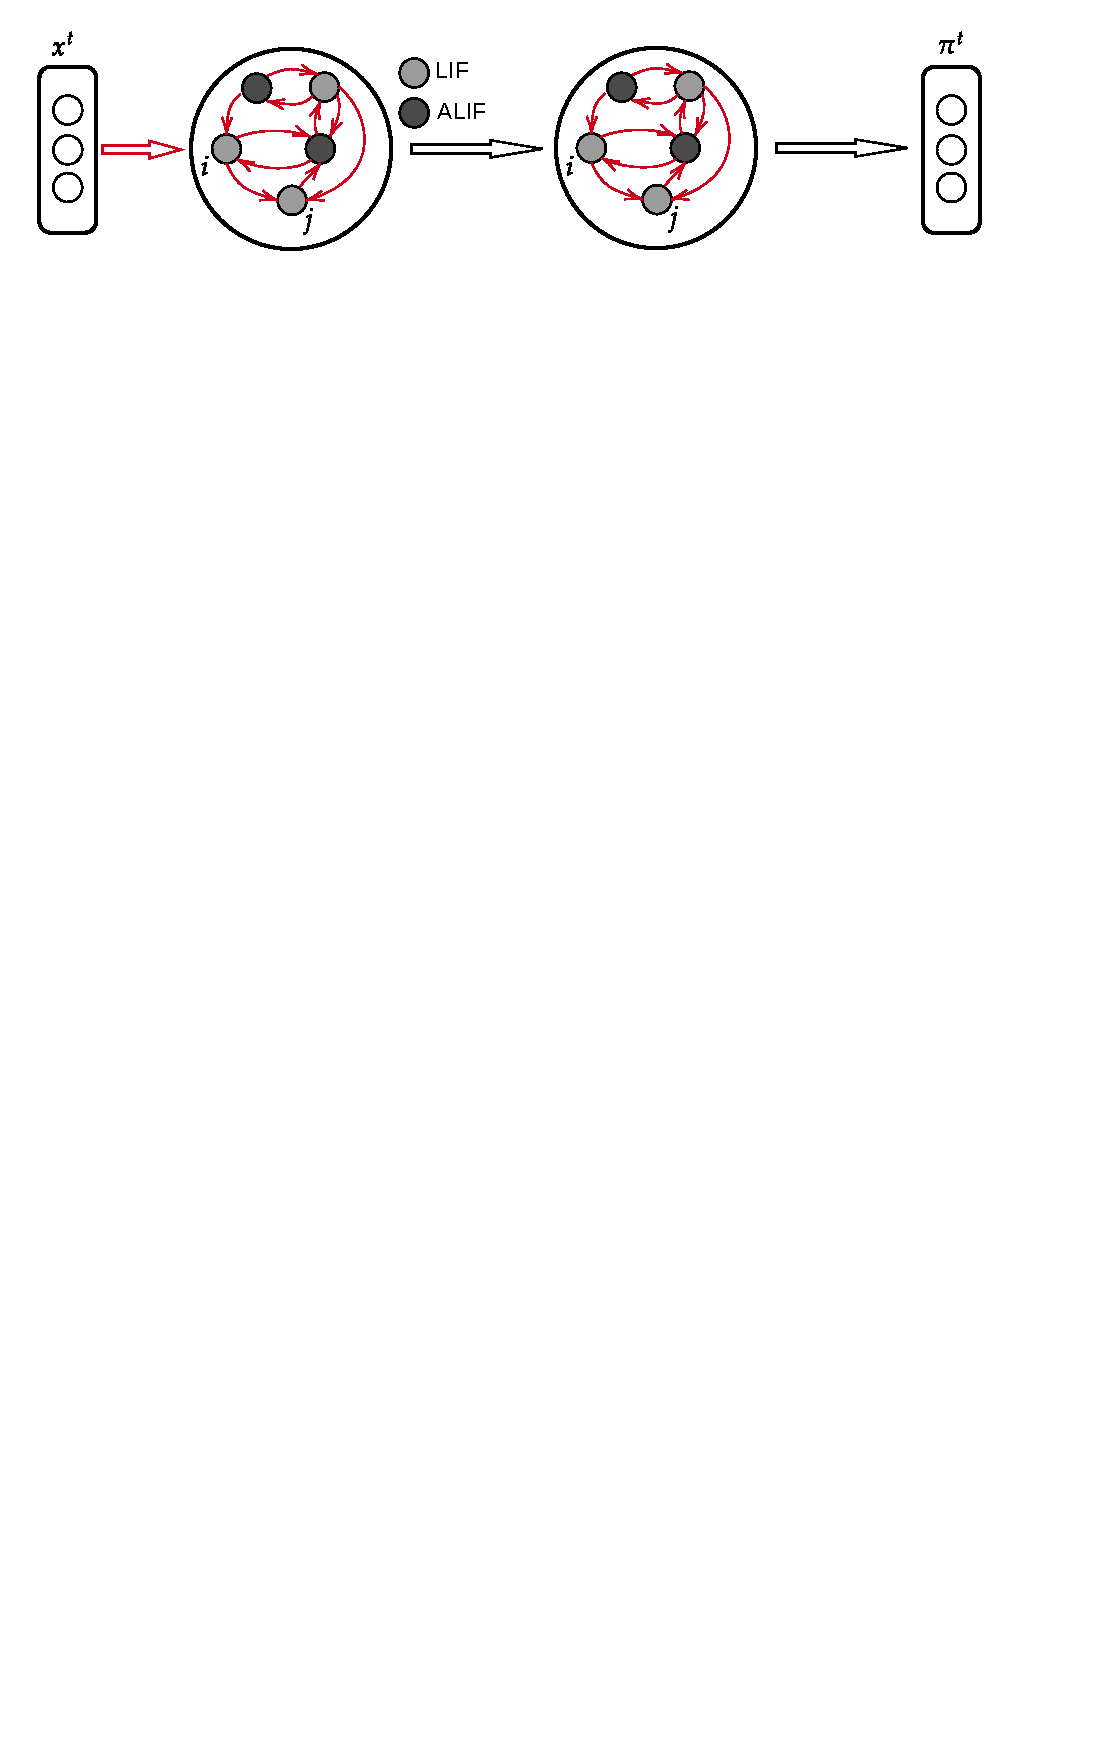
\includegraphics[trim=0 25cm 0 0, clip, width=\linewidth]{gfx/Multilayer}
		    \caption[Multi-layer illustration.]{An illustration of a multi-layer network architecture. Some details shown in Figure (\ref{fig:topology-sl} b) are omitted for clarity}
		    \label{fig:topology-ml}
		  \end{figure}

		The multi-layer e-prop architecture can be described in the same formal model as its single-layer counterpart, in which the hidden state is based on temporally (i.e., online) and spatially locally available information at a neuron $j$:

        \begin{equation}
        \mathbf{h}^t_j = M\left(\mathbf{h}_j^{t-1}, \mathbf{z}^{t-1}, \mathbf{x}^t, \mathbf{W}_j\right).\tag{\ref{eq:model} revisited}
        \end{equation}
        For the multi-layer architecture, however, neurons in deeper layers no longer depend on the input, but on the observable states of the previous layer at the same time step, such that at every time step, a full pass through the network is made.
        We modify the indexing notation accordingly, in order to directly refer to neurons and weights in a particular layer $r \in [1\mathrel{{.}\,{.}}\nobreak R]$:
        \begin{equation}\label{eq:ml_model}
        \mathbf{h}^t_{rj} = \begin{cases}
        M\left(\mathbf{h}_{rj}^{t-1}, \mathbf{z}_r^{t-1}, \mathbf{x}^t, \mathbf{W}_{rj}\right)       & \mbox{if } r = 1\\
        M\left(\mathbf{h}_{rj}^{t-1}, \mathbf{z}_r^{t-1}, \mathbf{z}_{r-1}^t, \mathbf{W}_{rj}\right) & \mbox{otherwise,}
        \end{cases}
        \end{equation}
        where $\mathbf{h}^t_{rj}$ (resp. $z^t_{rj}$) is the hidden state (resp. observable state) of a neuron $j$ in layer $r$. and $\mathbf{W}_{rj} = \mathbf{W}^\text{in}_{rj} \cup \mathbf{W}^\text{rec}_{rj}$ is the set of afferent weights to neuron $j$ in layer $r$.

        Similarly, the observable state can be modeled by
        \begin{equation}\label{eq:ml_model_obs}
        z^t_{rj} = f\left(\mathbf{h}_{rj}^t\right)
        \end{equation}
        and the network output by
        \begin{equation}
        y^t_k = \kappa y^{t-1}_k + \sum_{j,r}W^\text{out}_{rkj}z_{rj}^t + b_k,
        \end{equation}
        where $W^\text{out}_{rkj}$ is a weight between neuron $j$ in layer $r$ and output neuron $k$.
        Note that the summation over $r$ entails that the output layer is connected to all neurons in all layers in the network.
        This allows trainable broadcast weights in earlier layers, such as those found in symmetric and adaptive e-prop.

        \paragraph{Multi-layer ALIF neurons}
        An ALIF neuron in a multi-layer architecture is similar to one in a single-layer architecture (see Section \ref{sec:alif}).
        The only difference, apart from the layer indexing, is its activity update.
        For a multi-layer ALIF neuron, the activity value is given by
        \begin{equation}\label{eq:ml_alifV}
        v^{t+1}_{rj} = \alpha v_{rj}^t + \sum_{i\neq j}W^\text{rec}_{rji}z_i^t + \sum_i W^\text{in}_{rji}I - z_{rj}^tv_
        \text{th},
        \end{equation}
        where
        \begin{equation}\label{eq:inpVml}
        I = \begin{cases}
        	x^{t+1}_i       &\mbox{if } r = 1 \\
            z^{t+1}_{r-1,i} &\mbox{otherwise.}
            \end{cases}
        \end{equation}


	\subsection{Other neuron types}

		In this section, the STDP-ALIF and Izhikevich neuron models are presented.
		The advantage of these models over the standard ALIF model is that they naturally elicit STDP.
		Additionally, the Izhikevich model has an implicit refractory mechanism that is built into its system of equations, making it a more biologically plausible model, as opposed to the (STDP-)ALIF model that requires an explicit timer variable in a neuron's hidden state (but it is still local and online).

		The Izhikevich e-prop neuron model was first presented by \citet{traub2020learning} only in a single-synapse demonstration of its STDP properties.
		In this report, the performance of the e-prop Izhikevich model is experimentally validated in a learning task for the first time.
		\citet{traub2020learning} also described the STDP-LIF, which is a non-adaptive modification of the standard LIF neuron.
		Here, its adaptive counterpart, the STDP-ALIF model, is derived and validated as well.
		This allows for a direct comparison between the ALIF and STDP-ALIF models, such that the effects of STDP can be more precisely analyzed.

		\subsubsection{STDP-ALIF}
			The key change between the ALIF and STDP-ALIF neuron is that the latter is reset to zero at a spike event, and when its refractory period of $\delta t_\text{ref}$ time steps ends.
			Recall that in contrast, the standard ALIF neuron only uses a soft reset by including a term $-z^t_{rj}v_\text{th}$ in its activation update equation (Equation \ref{eq:ml_alifV}).

			The activation update of the STDP-ALIF neuron is therefore:
			\begin{equation}\label{eq:ml_stdpalifV}
	        v^{t+1}_{rj} = \alpha v_{rj}^t + \sum_{i\neq j}W^\text{rec}_{rji}z_i^t + \sum_i W^\text{in}_{rji}I -z^t_{rj}\alpha v^t_{rj} - z_{rj}^{t-\delta t_\text{ref}}\alpha v^t_{rj},
	        \end{equation}
	        where, again, $I$ is the network input if $r=1$, otherwise it is the observable state of neuron $i$ in the preceding layer (see Equation \ref{eq:inpVml}).
	        Recall that a neuron cannot spike for $T^\text{refr}$ time steps after its last spike---therefore, the neuron is still suppressed at time step $t-\delta t_\text{ref}$ and hence the fourth and fifth terms $-z^t_{rj}\alpha v^t_{rj}$ and $- z_{rj}^{t-\delta t_\text{ref}}\alpha v^t_{rj}$ cannot simultaneously be nonzero.
	        Note also that Equation \ref{eq:ml_stdpalifV} will not necessarily set the activation value precisely to 0 at spike time and after the refractory time, as only the activation that caused the neuron to spike will be subtracted, and the new input values described in its second and third term will be added to the new activation value.

	        The hidden state derivative changes accordingly:
	        \begin{align}
	        \frac{\partial v_{rj}^{t+1}}{\partial v^t_{rj}} &= \alpha - z^t_{rj}\alpha - \alpha z_{rj}^{t-\delta t_\text{ref}}\\
	        &= \alpha\left(1 - z^t_{rj} - z_{rj}^{t-\delta t_\text{ref}}\right).
	        \end{align}
	        Note that the absence of $a^t_{rj}$ in the new activation update entails that the other entries of the hidden state Jacobian are equal to those of the ALIF model, \ie, $\frac{\partial v^{t+1}_{rj}}{\partial a^t_{rj}}=0$, $\frac{\partial a^{t+1}_{rj}}{\partial v^t_{rj}}=\psi^t_{rj}$, and $\frac{\partial a^{t+1}_{rj}}{\partial a^t_{rj}} = \rho - \psi^t_{rj}\beta$.


	        Using these values, we compute the new eligibility trace:
	        \begin{align}
	        \bm{\epsilon}^{t+1}_{rji} &= \frac{\partial\mathbf{h}^{t+1}_{rj}}{\partial\mathbf{h}^t_{rj}}\cdot\bm{\epsilon}^t_{rji} + \frac{\partial\mathbf{h}^{t+1}_{rj}}{\partial W_{rji}}\\
	        &= \begin{pmatrix}
	        \alpha\left(1 - z^t_{rj} - z_{rj}^{t-\delta t_\text{ref}}\right)\epsilon_{rji, v}^t + z_{ri}^{t-1}\\
	        \psi^t_{rj}\epsilon^t_{rji, v} + \left(\rho - \psi^t_{rj}\beta\right)\epsilon^t_{rji,a}
	        \end{pmatrix}\label{eq:ml_stdpalif_evector}
	        \end{align}
	        Note that the observable state of the afferent neuron $z_{ri}^{t-1}$ in Equation \ref{eq:ml_stdpalif_evector} changes to $z_{r-1, i}^t$ if $\epsilon^{t+1}_{rji}$ corresponds to a weight between layer $r-1$ and $r$ and $r > 1$.
	        If the weight is instead between the network input and the first layer, then it changes to $x^t_i$.
	        Note also that this corrects an inconsistency in the STDP-LIF model described in \citet{traub2020learning}, where the observable state at the current time step $t$ is accessed instead of $t-1$, thereby diverging from the e-prop model in Equation \ref{eq:ml_model}.

	        The eligibility trace remains
	        \begin{align}
	        e^{t}_{rji} &= \frac{\partial z^{t}_{rj}}{\partial\mathbf{h}^{t}_{rj}} \cdot \bm{\epsilon}^{t}_{rji}\\
	        &= \psi^t_{rj}\left(\epsilon^t_{rji, v} - \beta\epsilon^t_{rji, a}\right).
	        \end{align}

	        By resetting the neuron activation at spike time and after the refractory time, STDP is introduced in the system by clamping the pseudo-derivative to a negative value, instead of 0, during the refractory time:

	        \begin{equation}
	        \psi^t_{rj} = \begin{cases}
	        -\gamma&\mbox{if } t - t_{z_{rj}} < \delta t_\text{ref}\\
	        \gamma\max\left(0, 1 - \left|\frac{v^t_{rj}-v_\text{th}}{v_\text{th}}\right|\right)&\mbox{otherwise}
	        \end{cases}
	        \end{equation}
	        The factor of the pseudo-derivative and the eligibility vector can therefore produce both positive or negative eligibility traces and gradients (see Figure \ref{fig:stdpalif}).

	        \begin{figure}[!ht]
	            \centering
	            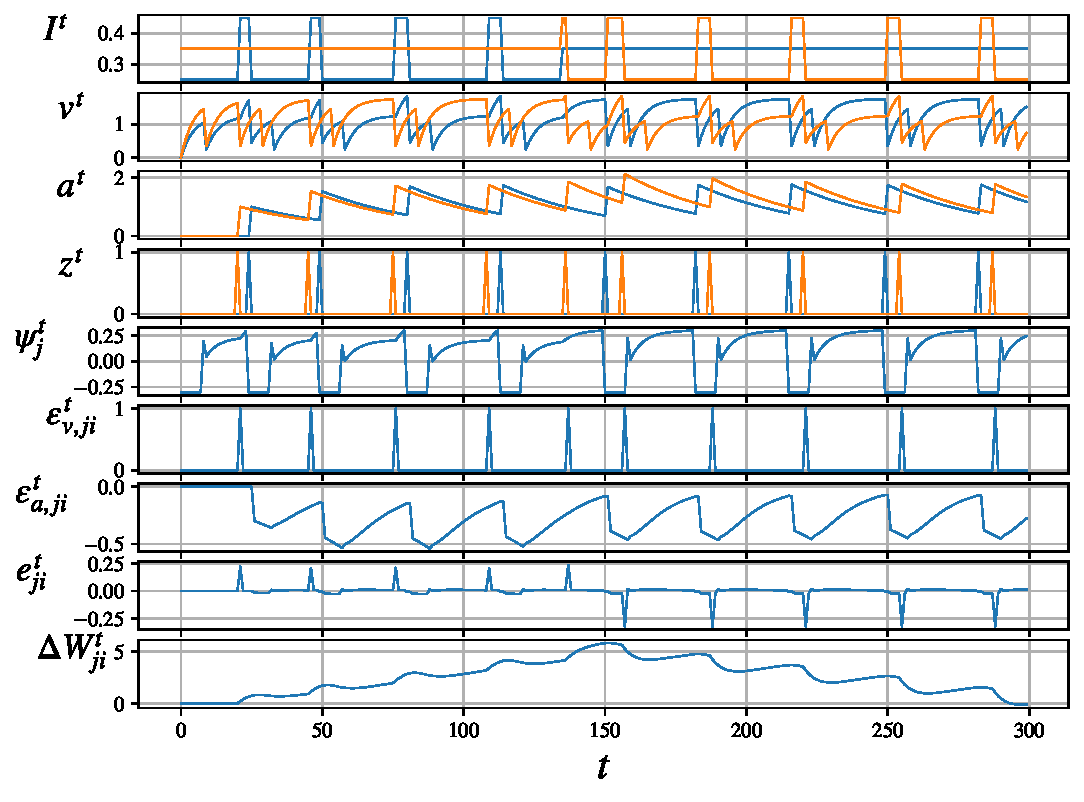
\includegraphics[width=\linewidth]{gfx/stdpalif}
	            \caption{A single-synapse demonstration of the STDP-ALIF.}
	            \label{fig:stdpalif}
	        \end{figure}

		\subsubsection{Izhikevich neuron}\label{sec:izhikevich}

			The standard system of equations of the Izhikevich neuron is described by
			\begin{align}
			v' &= 0.04v^2 + 5v + 140 - a + I\\
			a' &= 0.004v - 0.02a,
			\end{align}
			where $v'$ and $a'$ are the values of the activation value $v$ and recovery variable $a$ at the next time point, and $I$ is the current input to the neuron.
			Following \citet{traub2020learning}, the activation reset and refractory period are built into this system of equations by replacing $v$ and $a$ by respectively:
			\begin{align}
			\tilde{v}^t_{rj} &= v^t_{rj} - \left(v^t_{rj} + 65\right)z^t_{rj}\\
			\tilde{a}^t_{rj} &= a^t_{rj} + 2z^t_{rj},
			\end{align}
			such that when a spike event occurs (\ie, $z^t_{rj} = 1$), the activation value is reset to its baseline value of $-65$, and the recovery variable increases by 2.
			We describe this ``self-resetting'' Izhikevich neuron in the context of multi-layer e-prop as follows:
			\begin{align}
			v^{t+1}_{rj} &= \tilde{v}^t_{rj} + 0.04\left(\tilde{v}^t_{rj}\right)^2 + 5\tilde{v}^t_{rj} + 140 - \tilde{a}^t_{rj} + I^t_{rj}\\
			a^{t+1}_{rj} &= \tilde{a}^t_{rj} + 0.004\tilde{v}^t_{rj}-0.02\tilde{a}^t_{rj}.
			\end{align}
			The partial derivatives of the hidden state $\mathbf{h}^t_{rj}$ can then be computed:
			\begin{align}
			\frac{\partial v^{t+1}_{rj}}{\partial v^t_{rj}} &= \left(1-z^t_{rj}\right)\left(6+0.08v^t_{rj}\right)\\
			\frac{\partial a^{t+1}_{rj}}{\partial v^t_{rj}} &= -1\\
			\frac{\partial v^{t+1}_{rj}}{\partial a^t_{rj}} &= 0.004\left(1-z^t_{rj}\right)\\
			\frac{\partial a^{t+1}_{rj}}{\partial a^t_{rj}} &= 0.98.
			\end{align}

			Using these values, we compute the new eligibility trace:
	        \begin{align}
	        \bm{\epsilon}^{t+1}_{rji} &= \frac{\partial\mathbf{h}^{t+1}_{rj}}{\partial\mathbf{h}^t_{rj}}\cdot\bm{\epsilon}^t_{rji} + \frac{\partial\mathbf{h}^{t+1}_{rj}}{\partial W_{rji}}\\
	        &= \begin{pmatrix}\left(1-z^t_{rj}\right)\left(6+0.08v^t_{rj}\right)\epsilon^t_{rji, v} -\epsilon^t_{rji, a} + z_{ri}^{t-1}\\
	        0.004\left(1-z^t_{rj}\right)\epsilon^t_{rji, v} + 0.98\epsilon^t_{rji, a}
	        \end{pmatrix}\label{eq:ml_izhikevich_evector}
	        \end{align}
	        As in \citet{traub2020learning}, the pseudo-derivative is defined as
	        \begin{equation}
	        \psi^t_{rj} = \gamma\ \exp\left(\frac{\min\left(v^t_{rj}, 30\right) - 30}{30}\right),
	        \end{equation}
	        such that
	        \begin{equation}
	        \begin{pmatrix}\frac{\partial z^t_{rj}}{\partial v^t_{rj}}\\\frac{\partial z^t_{rj}}{\partial u^t_{rj}}\end{pmatrix}
	        = \begin{pmatrix}\psi^t_{rj}\\0\end{pmatrix}
	        \end{equation}
	        and therefore only $\epsilon^t_{rji, v}$ is used in computing the eligibility trace:
	        \begin{align}
	        e^t_{rji} &= \left(\psi^t_{rj}\ 0\right)\begin{pmatrix}\epsilon^t_{rji, v}\\\epsilon^t_{rji, a}\end{pmatrix} \\
	        &= \psi^t_{rj}\epsilon^t_{rji, v}.
	        \end{align}

	    However, when inserting these equations in a single-synapse demo, the eligibility vector assumes extremely high or low values (see Figure \ref{fig:demo_izh}).

		\begin{figure}[ht]
		    \centering
		    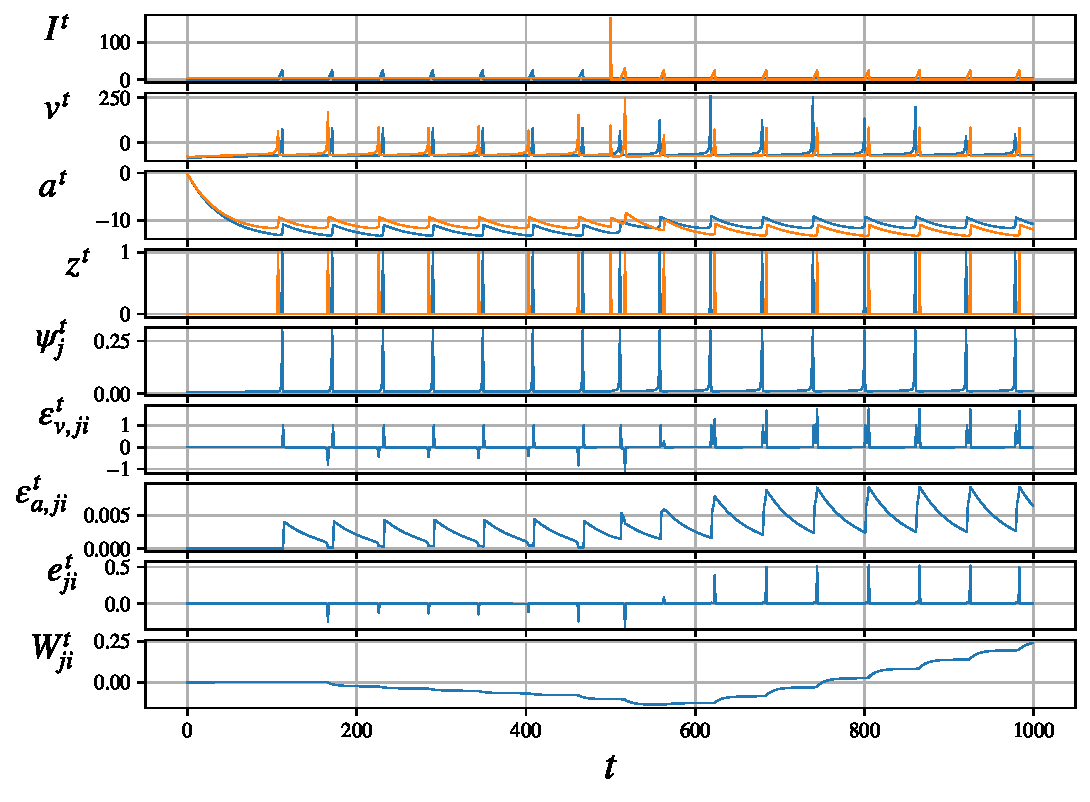
\includegraphics[width=\linewidth]{gfx/demo_izh}
		    \caption[A single-synapse demo of the uncorrected Izhikevich neuron.]{A single-synapse demo of the uncorrected Izhikevich neuron. Note that $\epsilon^t_{ji, v}$ takes on extreme values and that the eligibility vector flips sign at any pair of spikes.}
		    \label{fig:demo_izh}
		\end{figure}

	    This suggests that the Izhikevich neuron does not fit the e-prop framework well.
	    In this report, this is corrected by clipping the value of $\epsilon^t_{ji,v}$ to $\left[-3, 3\right]$ and $\epsilon^t_{ji,a}$ to $\left[-0.005, 0.005\right]$.
	    This correction yields the desired STDP behavior (see Figure \ref{fig:demo_izh_corrected}).

        \begin{figure}[ht]
            \centering
            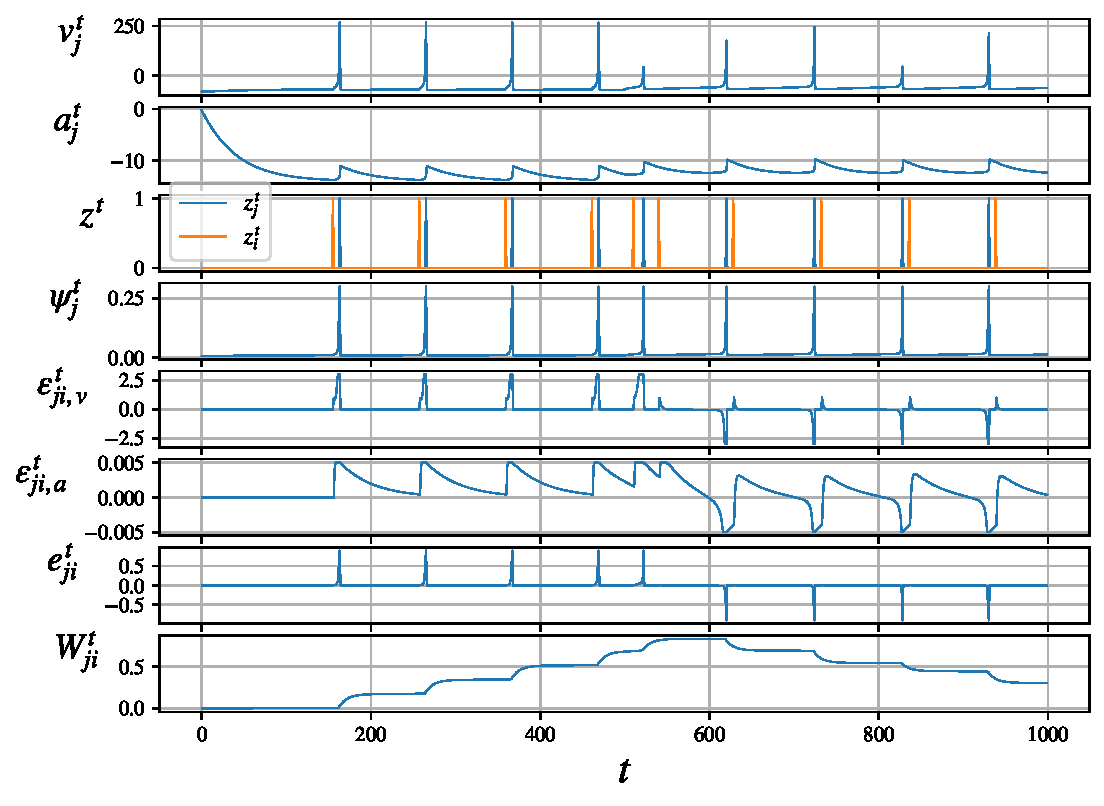
\includegraphics[width=\linewidth]{gfx/demo_izh_corrected}
            \caption{A single-synapse demo of the corrected Izhikevich neuron.}
            \label{fig:demo_izh_corrected}
        \end{figure}


\section{Regularization}

	Firing rate regularization and L2 regularization are applied to improve the stability of the learning process and the generalizability of the resulting model.
	These two regularization methods are motivated by biological plausibility, ease of implementation in the e-prop framework, and improved empirical performance.

	\subsection{Firing rate regularization}
		A firing rate regularization term is added to individually control the spike frequencies of the neurons.
		Since spikes in a neuromorphic architecture cost energy, the practical motivation for this regularization term is that it increases the energy efficiency of the model.
		The biological motivation is that the firing rate of biological neurons is also under homeostatic control \citep{erickson2006activity}.

		Firing rate is implemented by adding a regularization term $E_\text{reg}$ to the loss function that penalizes neurons that have a firing rate that is too low or too high:
		\begin{equation}
			E_\text{reg} = \frac{1}{2}\sum_j\left(f^\text{target} - f^{\text{av}, t}_{rj}\right)^2,
		\end{equation}
		where $f^\text{target}$ is a target firing rate of \SI{10}{\Hz}, and
		\begin{equation}
		f^{\text{av},t}_{rj} = \frac{1}{t} z^{\text{total},t}_{rj}
		\end{equation}
		is the running average spike frequency, where $z^{\text{total},t}$ accumulates spikes emitted by neuron $j$ in layer $r$ up to (and including) time step $t$.
		Note that $z^{\text{total},0} = 0$, \ie, the accumulation resets at each new training sample.
		By implementing this sum as a hidden variable, e-prop remains an online and local training algorithm when firing rate regularization is implemented.
		Adhering to these two constraints supports the biological plausibility of the firing rate regularization term.
		After the training sample, the effect of the firing rate regularization on the weight update is integrated.

		Another possibility to compute the average firing rate would be to track an exponentially decaying firing rate.
		This was not implemented in this research for the following two reasons. First, the effects of the firing rate regularization are integrated only at the end of a training sample (see Equation \ref{eq:deltareg}), likely causing any fluctuations of the average frequency over time to cancel each other out and result in an effectively similar regularization term as the current, non-decaying frequency calculation.
		Second, since one of the objectives of this research is to reproduce results obtained \citet{bellec2020solution} and expand on that paper, the regularization term is kept as true to it as possible.
		However, analyzing the effects of different firing rate regularization terms might be an interesting direction for future research.

		To insert the regularization term into the e-prop framework, we compute the weight update that regularizes the firing rate toward $f^\text{target}$ through gradient descent, similarly to the main e-prop weight update (Equation \ref{eq:eprop_grd}):
		\begin{equation}
		\frac{\partial E_\text{reg}}{\partial z_{rj}^t} = \left(f^\text{target} - f^{\text{av}, t}_{rj}\right).
		\end{equation}
		Note that this regularization loss differs from the firing rate regularization described in \citet{bellec2020solution}, in which the firing rate is calculated in an offline fashion, by retroactively computing the average firing rate based on all spikes instead of only accumulated spikes.
		Note also that in \citet{bellec2020solution}, $\frac{\partial E_\text{reg}}{\partial z_{rj}^t}$ is multiplied with the eligibility trace $e^t_{rji}$, as in Equation \ref{eq:eprop_grd} to obtain the weight update, whereas in this report, the eligibility trace is omitted, resulting in a number of benefits:
		\begin{enumerate}
			\item It allows silent neurons that have infrequently spiking afferent neurons to more easily increase their firing rate, because their low afferent eligibility traces no longer nullifies the regularization gradient, and thereby results in a better empirical learning performance;
			\item It is more efficient in emulations on von Neumann machines, because the element-wise multiplication of $\frac{\partial E_\text{reg}}{\partial z_{rj}^t}$ and the eligibility trace is a relatively large computation on the order $\Theta\!\left(n^2\right)$ that no longer needs to be computed.
			\item It is more intuitive, as only the gradient of the firing rate is used to compute the weight update.
		\end{enumerate}
		We apply the weight update $\Delta W_{rji}$ of the regularization gradient using
		\begin{equation}\label{eq:deltareg}
		\Delta_\text{reg} W_{rji} = -\eta\ c_\text{reg}\sum_t\left(f^\text{target} - f^{\text{av}, t}_{rj}\right).
		\end{equation}
		Note that the regularization gradients can be combined and accumulated over time on the same synaptic variable as the normal gradients, facilitating practical implementation of the learning procedure in both software emulations and neuromorphic embeddings:
		\begin{equation}
		\Delta W_{rji} = -\eta\ \sum_t\left(c_\text{reg}\left(f^\text{target} - f^{\text{av}, t}_{rj}\right) + L^t_{rj}\cdot\bar{e}^t_{rji}\right).
		\end{equation}

	\subsection{L2 regularization}
		To regularize weights around 0, a small fraction (parametrized by $c_\text{L2}$) of the value of the weight is added to its gradient value at every weight update:
		\begin{equation}
		\Delta_\text{L2} W_{rji} = -\eta\ c_\text{L2} \cdot W_{rji},
		\end{equation}
		which can be added to the full weight update as an extra term:
		\begin{equation}
		\Delta W_{rji} = -\eta\left(c_\text{L2} \cdot W_{rji} + \sum_t\left(c_\text{reg}\left(f^\text{target} - f^{\text{av}, t}_{rj}\right) + L^t_{rj}\cdot\bar{e}^t_{rji}\right)\right).
		\end{equation}
		The statistical motivation for this extra regularization term is that by softly restricting the weights, the network is less likely to overfit on the training data.

		The biological motivation is that biological synapses are regularized by a multiplicative factor to decrease the strength of individual synapses to the same proportion \citep{turrigiano2000hebb}, likely counteracting the run-away effects that the positive feedback of STDP naturally induces \citep{siddoway2014molecular}.
		Moreover, there are natural bounds of the strength of a biological synapse, measured by the amplitude of the postsynaptic potential, because the number of neurotransmitter vesicles and release sites is physically limited \citep{del1954quantal}.
		These natural limits are approximately \SI{0.4}{\mV} to \SI{20}{\mV} \citep{diaz2006target}.


% \section{Bidirectional network}
% 	\begin{tcolorbox}[colback=orange]
% 	- I/A
% 	- What, why, how?

% 	\end{tcolorbox}

\section{Optimizer}\label{sec:adam}

	For simplicity, in this report weight updates are described using stochastic gradient descent:
	\begin{equation}
		\Delta W_{rji} = -\eta \sum_t L^t_{rj}\cdot\bar{e}^t_{rji}.
	\end{equation}
	However, the results described in Chapter \ref{ch:results} are obtained using Adam (or Adaptive Moment Estimation) \citep{kingma2014adam}.
	This optimization method tracks running averages of the gradient and its second moment (resp. $M_{rji}$ and $V_{rji}$), and fits the local and online constraints of e-prop, because the running averages are tracked per individual synapse.
	The Adam weight update in the context of multi-layer e-prop is given by:
	\begin{align}
	M_{rji}^{(i+1)} &= \beta_1 M_{rji}^{(i)} + \left(1 - \beta_1\right)G^{(i)}_{rji} \\
	V_{rji}^{(i+1)} &= \beta_2 V_{rji}^{(i)} + \left(1 - \beta_2\right)\left(G^{(i)}_{rji}\right)^2 \\
	\widehat{M}_{rji} &= \frac{M_{rji}^{(i+1)}}{1 - \beta_1^{i+1}} \\
	\widehat{V}_{rji} &= \frac{V_{rji}^{(i+1)}}{1 - \beta_2^{i+1}} \\
	\Delta W_{rji}^{(i+1)} &= -\eta \frac{\widehat{M}_{rji}}{\sqrt{\widehat{V}_{rji}} + 10^{-5}},
	\end{align}
	where $G^{(i)}$ is the estimated gradient $\sum_t L^t_{rj}\cdot\bar{e}^t_{rji}$ at weight update $i$, and $\beta_1=0.9$ and $\beta_2=0.999$ are the forgetting factors for the gradient and its second moment, respectively.
	The firing rate and L2 regularization terms are omitted here for clarity.
	Note that the forgetting factors are not indexed, but raised to the power of $i+1$, in computing the bias-corrected estimates $\widehat{M}_{rji}$ and $\widehat{V}_{rji}$.
	Note also that minibatches of size 32 are used to more accurately estimate the gradient and enable a stabler descent in the error landscape.
	The value of $G^{(i)}_{rji}$ is computed as the mean over the minibatch.

	Note that the learning rate is linearly ramped up from 0 to $\eta$ during the first epoch, such that the initial minibatches are used to aggregate good initial momentum buffers, as the variance is higher when fewer minibatches are processed.
	This ``warming up'' of the learning rate is a variance reduction technique that has shown beneficial results in training other models \citep{liu2019variance}.
	Empirical observations on the resulting learning curves (see Chapter \ref{ch:results}) suggest that this procedure does not obstruct a rapid initial decrease of the loss function.
